\documentclass{beamer}
\usepackage{outlines}
\usepackage{beamerthemeIlmenau}
\usepackage{amsthm,amssymb}
\usepackage{mathrsfs}
\usepackage{amsmath,amscd}
\usepackage[mathscr]{euscript}
\usepackage{fontawesome}

\usefonttheme[onlymath]{serif}
\usecolortheme{dolphin}
\definecolor{ButlerLBlue}{HTML}{b48484}
\definecolor{ButlerLGreen}{HTML}{58dbe0}
\usepackage{ragged2e}

%\setbeamercolor{structure}{fg=ButlerLBlue}
%\setbeamercolor{background canvas}{bg=black}
\setbeamercolor{normal text}{fg=ButlerLBlue}
\setbeamercolor{section in head/foot}{bg=ButlerLBlue}
\setbeamercolor{mini frame}{bg=ButlerLBlue}
\setbeamercolor{title}{fg=ButlerLBlue}
\setbeamercolor{frametitle}{fg=ButlerLBlue}


\setbeamercolor{section in head/foot}{fg=black}

\setbeamercolor{subsection in head/foot}{bg=ButlerLGreen}
\setbeamercolor{subsection in head/foot}{fg=black}

\setbeamercolor{institute in head/foot}{fg=black}
\makeatletter
%change the `footline' template to include frame numbers
\setbeamertemplate{section in head/foot}{%
  \parbox[c][0.33cm][t]{\dimexpr(\textwidth-1.3cm)/\beamer@sectionmax\relax}{%
    \RaggedRight\fontsize{4}{4}\selectfont\insertsectionhead}}

\defbeamertemplate*{footline}{myminiframes theme}
  {%
    \begin{beamercolorbox}[colsep=1.5pt]{upper separation line foot}
    \end{beamercolorbox}
    \begin{beamercolorbox}[ht=2.5ex,dp=1.125ex,%
      leftskip=.3cm,rightskip=.3cm plus1fil]{author in head/foot}%
      \leavevmode{\usebeamerfont{author in head/foot}\insertshortauthor}%
      \hfill%
     
    \end{beamercolorbox}%
    \begin{beamercolorbox}[ht=2.5ex,dp=1.125ex,%
      leftskip=.3cm,rightskip=.3cm plus1fil]{title in head/foot}%
      {\usebeamerfont{title in head/foot}\insertshorttitle\hfill \insertframenumber/\inserttotalframenumber}%<-here
    \end{beamercolorbox}%
    \begin{beamercolorbox}[colsep=1.5pt]{lower separation line foot}
    \end{beamercolorbox}
  }
\makeatother

%change look of sections in ToC
\defbeamertemplate*{section in toc}{mysections in toc}
{\leavevmode ---\,\inserttocsection\par}

%change look of subsections in ToC
\defbeamertemplate*{subsection in toc}{mysections in toc}
{\leavevmode\leftskip=2.5em --\,\inserttocsubsection\par}
%%%%%in header:
\usepackage{tikz}
\usetikzlibrary{matrix}
\usetikzlibrary{shapes,arrows}

%\usepackage{multicol}

\setbeamertemplate{navigation symbols}{}
\definecolor{pastgrey}{rgb}{0.81, 0.84, 0.78}
\definecolor{spink}{rgb}{0.92, 0.73 , 0.72}
\setbeamercolor{block title}{bg=ButlerLGreen} %color for proof and theorems
\definecolor{PicBlue}{rgb}{0.19, 0.74 , 0.92}
\usepackage{listings}
\usepackage{color}

% \usepackage{inconsolata}

% \usepackage{ccfonts}
% \usepackage[T1]{fontenc}
% %\usepackage{antpolt}
% \usepackage{fontenc}

\definecolor{dkgreen}{rgb}{0,0.6,0}
\definecolor{gray}{rgb}{0.5,0.5,0.5}
\definecolor{mauve}{rgb}{0.58,0,0.82}
\lstdefinelanguage{JavaScript}{
  morekeywords=[1]{break, continue, delete, else, for, function, if, in,
    new, return, this, typeof, var, void, while, with},
  % Literals, primitive types, and reference types.
  morekeywords=[2]{false, null, true, boolean, number, undefined,
    Array, Boolean, Date, Math, Number, String, Object},
  % Built-ins.
  morekeywords=[3]{eval, parseInt, parseFloat, escape, unescape},
  sensitive,
  morecomment=[s]{/*}{*/},
  morecomment=[l]//,
  morecomment=[s]{/**}{*/}, % JavaDoc style comments
  morestring=[b]',
  morestring=[b]"
}[keywords, comments, strings]
\lstset{
  basicstyle=\tiny\ttfamily,
  language=C++,
  aboveskip=3mm,
  belowskip=3mm,
  showstringspaces=false,
  columns=flexible,
  numbers=left,
  numberstyle=\tiny\color{gray},
  keywordstyle=\color{blue},
  commentstyle=\color{dkgreen},
  stringstyle=\color{mauve},
  breakatwhitespace=true,
  tabsize=3
}

%\setbeamercolor{block body}{bg=pastgrey}
%\setbeamercolor{block body}{fg=ButlerLBlue}

\newcommand\T{\rule{0pt}{2.6ex}}
\newcommand\B{\rule[-1.2ex]{0pt}{0pt}}


\newcommand{\Tau}{\mathrm{T}}

%\theoremstyle{plain}
\newtheorem{thm}{Theorem}[section]
\newtheorem{cor}[thm]{Corollary}
\newtheorem{lem}[thm]{Lemma}
\newtheorem{prop}[thm]{Proposition}
\usepackage{parcolumns}

%\newtheorem{cor}{Corollary}
%\newtheorem*{prop*}{Proposition}

\theoremstyle{definition}
\newtheorem{defn}[thm]{Definition}

\newtheorem{quest}{Question}
\newtheorem{facts}{Facts}
\newtheorem{blank}{}

\newcommand{\norm}[1]{\left\Vert#1\right\Vert}
\newcommand{\abs}[1]{\left\vert#1\right\vert}
\newcommand{\set}[1]{\left\{#1\right\}}
\newcommand{\ip}[1]{\left\langle#1\right\rangle}
\newcommand{\ds}{\displaystyle}
\newcommand{\p}[1]{\left(#1\right)}
\renewcommand{\qedsymbol}{$\blacksquare$}
\usepackage{charter}
\usepackage{multirow}
\usepackage[normalem]{ulem}
\useunder{\uline}{\ul}{}
\title{Command Line Wizardry}
\author[Troy]{Troy Wiegand}
\date{\today}
\institute{Butler University}


    \usepackage{xargs}

\begin{document}

\frame{\titlepage}


\begin{frame}
    \frametitle{Shells We Are Going to Talk About}

    \pause 

    \begin{center}
    \textbf{\Huge csh VS bash VS zsh}
    \end{center}

\end{frame}


\begin{frame}
    \frametitle{History Lesson}
    \begin{center}
    \textbf{\huge \only<2>{1979 Stephen R. Bourne} \only<3>{Bourne Shell (sh)} \only<4>{"Tenex" C Shell (csh/tcsh)} \only<5>{Bourne Again Shell (bash)} \only<6>{Z Shell (zsh)} \only<7>{Pretty Family Tree}}\\
    \vspace{.3in}
    \only<2>{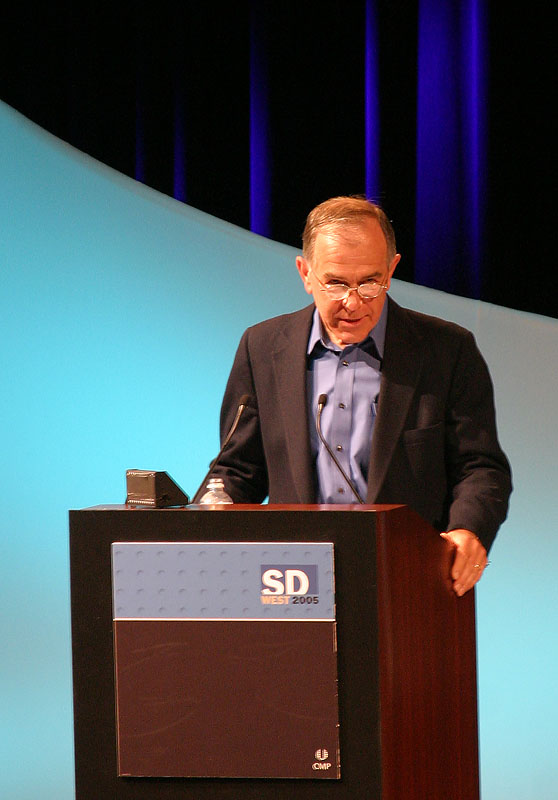
\includegraphics[scale=.3]{Steve_Bourne.jpg}}
    \only<3>{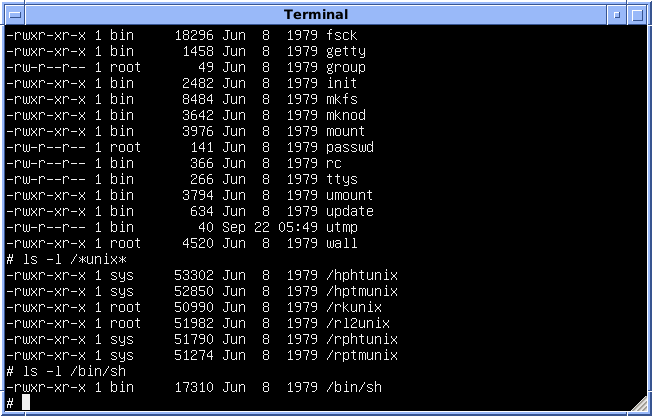
\includegraphics[scale=.3]{sh.png}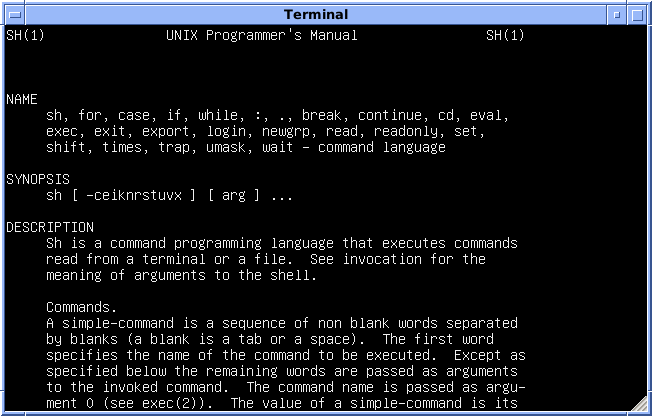
\includegraphics[scale=.3]{man_sh.png}}
        \only<4>{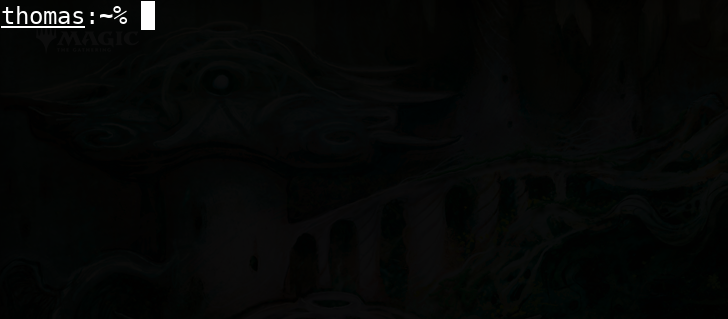
\includegraphics[scale=.3]{thomascsh.png}}
    \only<5>{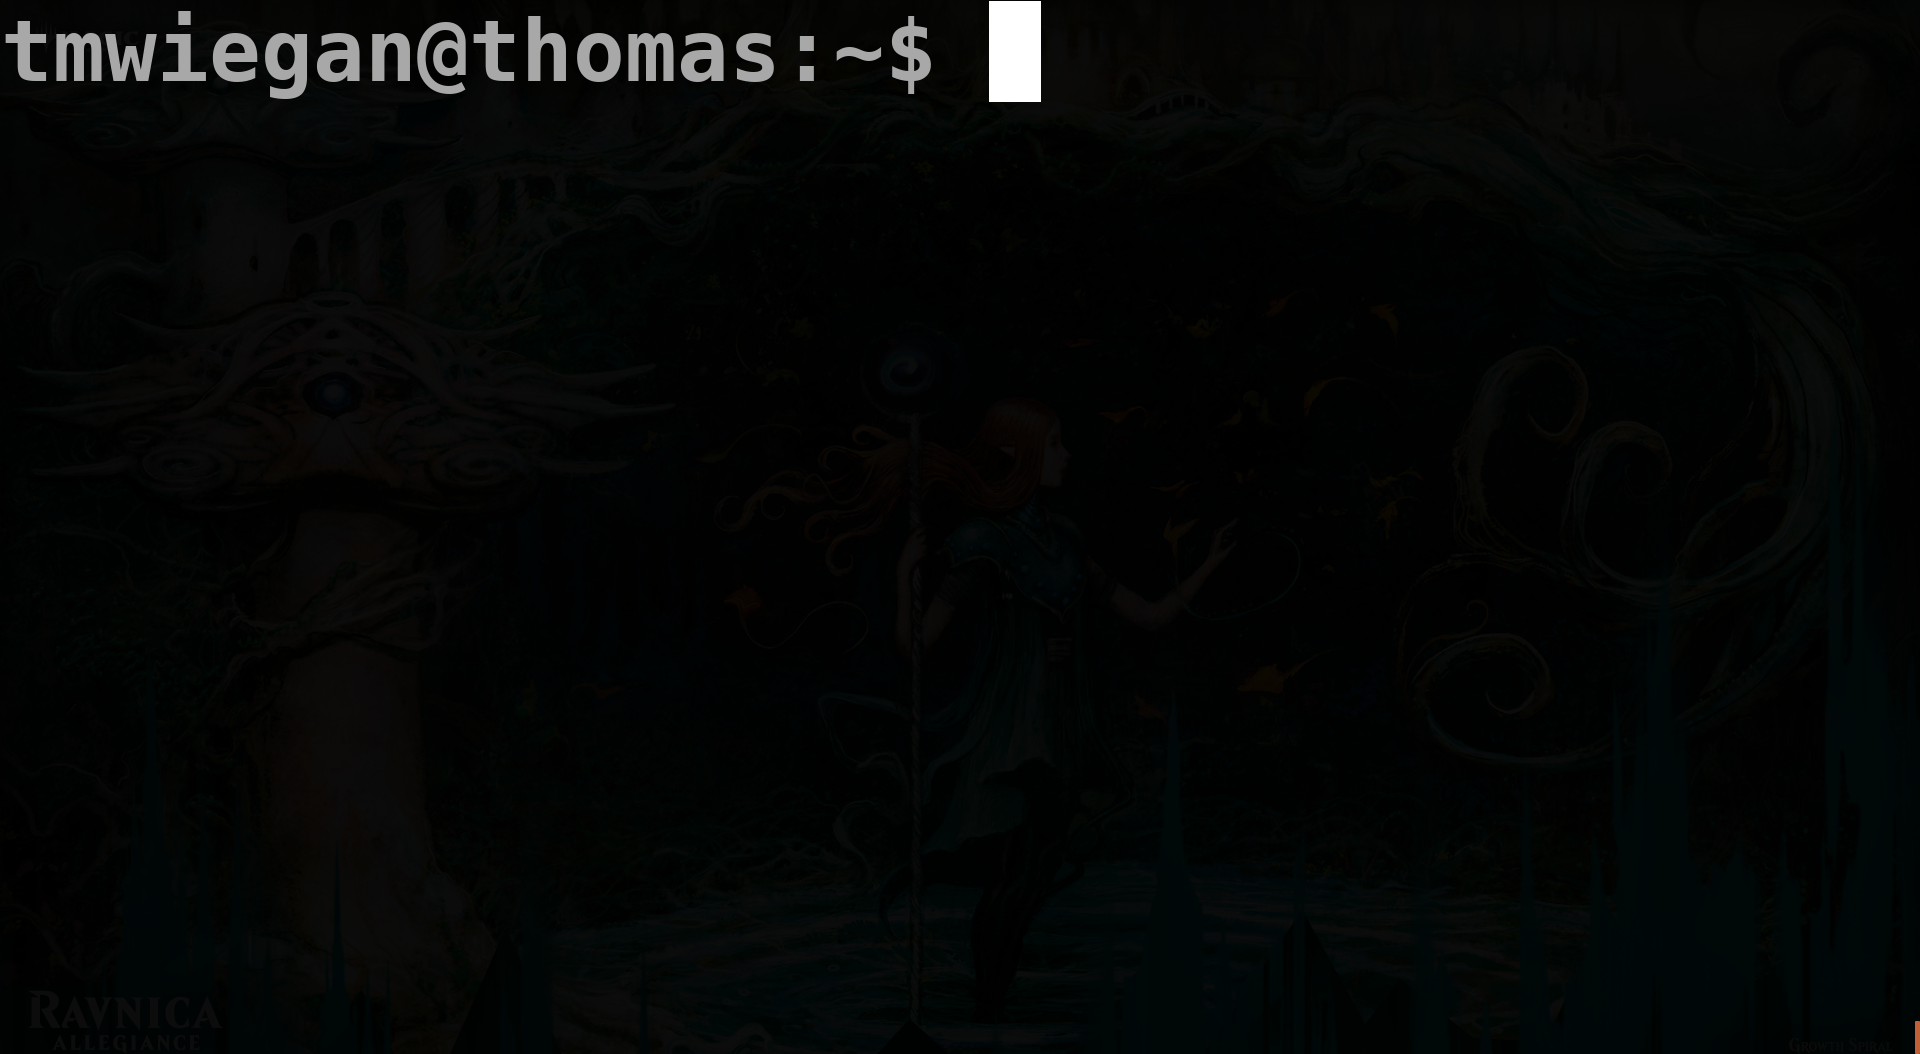
\includegraphics[scale=0.15]{thomasbash.png}}
    \only<6>{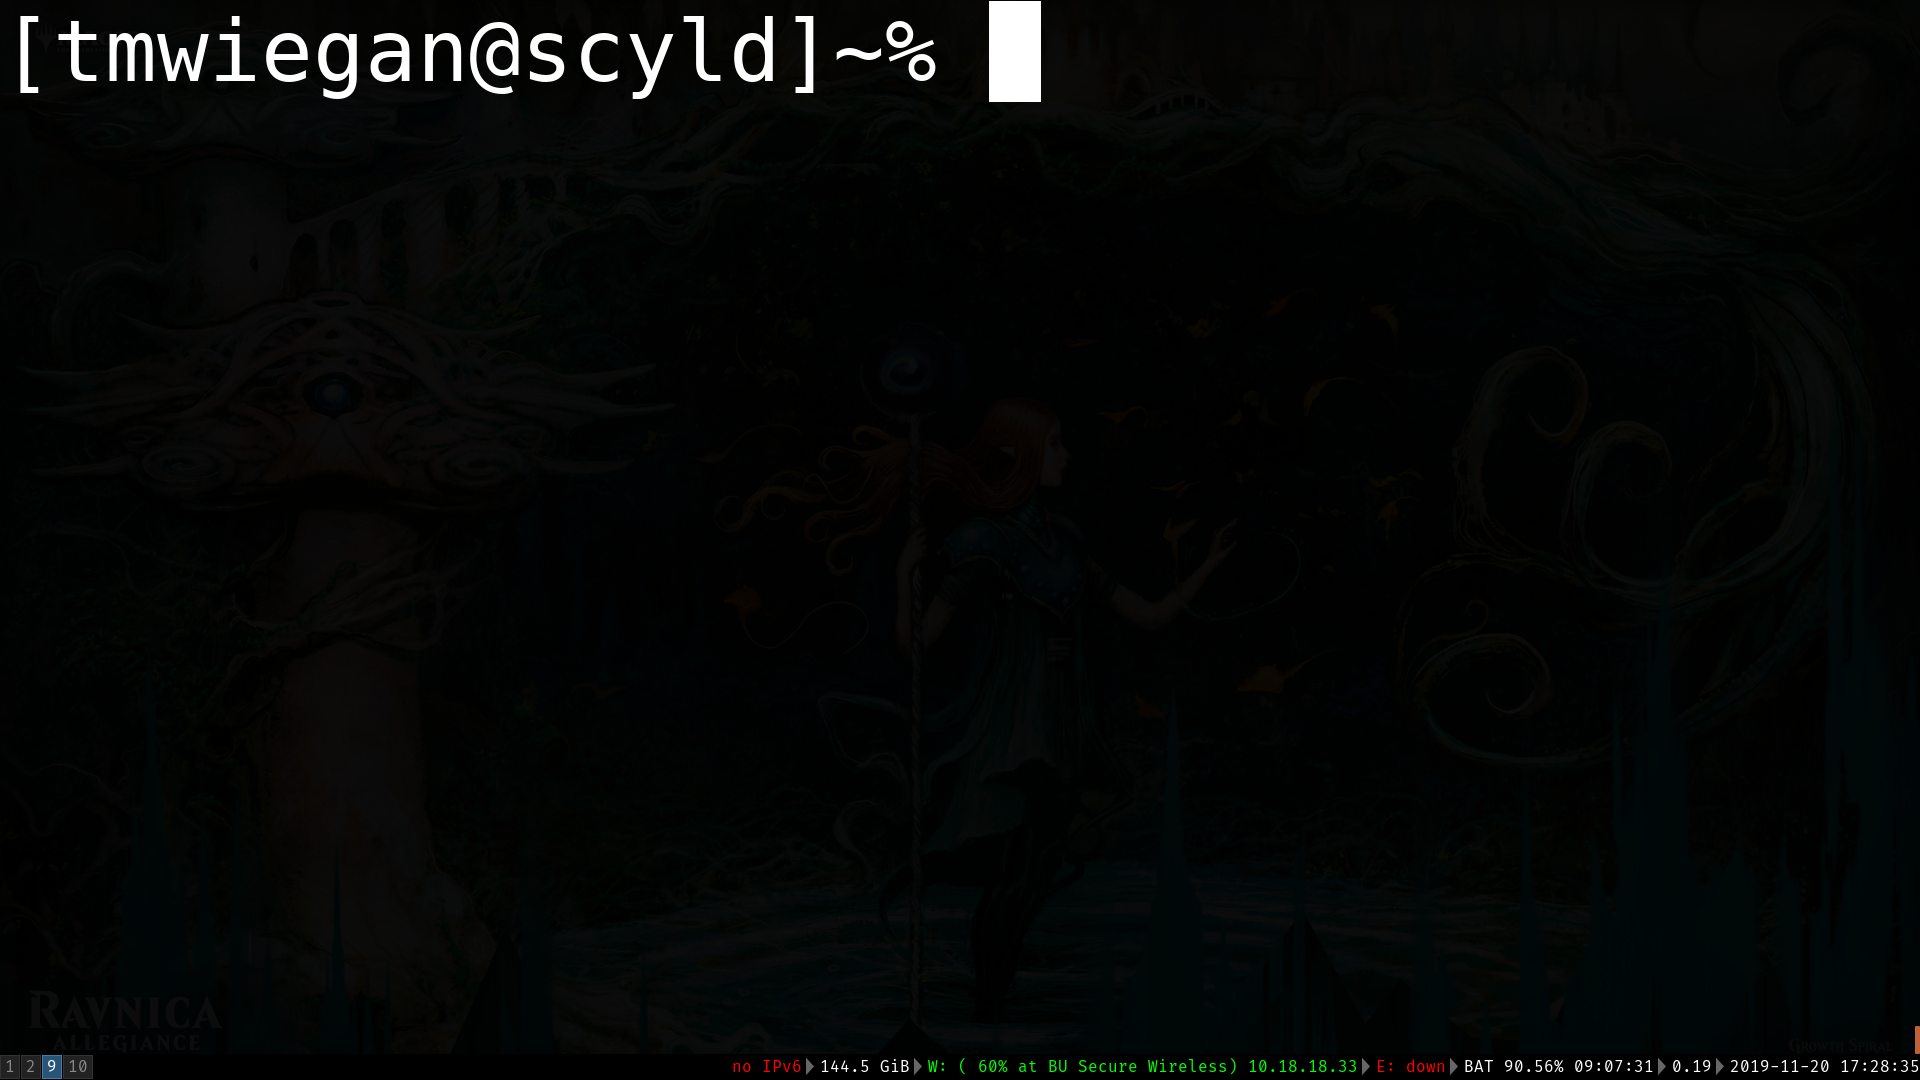
\includegraphics[scale=0.15]{bigdawgzsh.png}}
    \only<7>{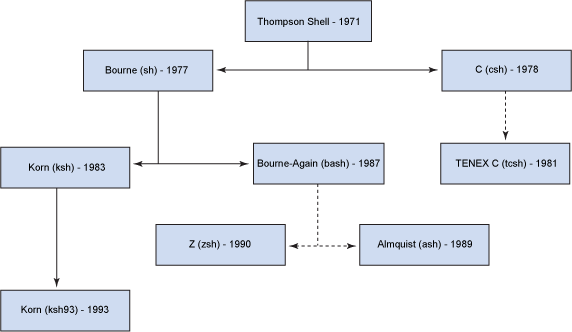
\includegraphics[scale=0.4]{familytree.png}}
    \end{center}
\end{frame}


\begin{frame}
  \Large
  \frametitle{\huge Why Is It Called That?}

  \begin{itemize}
  \pause

  \item Computer Scientists are super big lame-o's historically.

  \pause

  \item Storage was small

  \pause 

  \item Names needed to be as well

  \end{itemize}

\end{frame}

\begin{frame}
  \frametitle{\huge Anatomy of a Command}
\pause
  \large
\begin{center}
\$ \pause program\_name \uncover<4->{ -a --options } \pause list of arguments
  \end{center}

\begin{itemize}
  \item The program we are trying to run is called program\_name
  \item The arguments are list, of, and arguments.
  \item The program is run with the options a and options
\end{itemize}

 \end{frame}

\end{document}